\section{Passwörter}
\begin{frame}{Passwörter}
  \visible<+->{Wer hat mindestens fünf Online-Accounts?}

  \visible<+->{Wer hat dafür mindestens drei verschiedene Passwörter?}

  \visible<+->{Wer beachtet, Passwörter nur über HTTPS einzugeben?}
\end{frame}

\begin{frame}{Anzahl Passwörter}
  \begin{itemize}
    \item Kundendaten gehen häufig verloren
    \begin{itemize}
      \item Schaden lässt sich begrenzen, wenn Benutzername und Passwort nur bei diesem einen Anbieter passen
    \end{itemize}
    \item Besonders wichtig: E-Mail-Accounts
    \begin{itemize}
      \item Weil ,,Passwort zurücksetzen`` oft via E-Mail
      \item Wer den E-Mail Account übernommen hat,\\ kann dadurch sämtliche Accounts übernehmen
    \end{itemize}
    \item Ideal: Jedes Passwort nur einmal verwenden
    \item Alternative: Passwörter ,,salzen``
    \begin{itemize}
      \item \textit{passwort}.amz für Onlineshop a
      \item \textit{passwort}.zal für Onlineshop z
      \item \textit{anderespasswort} für Mails
    \end{itemize}
  \end{itemize}
\end{frame}

\begin{frame}{Passwort Wiederverwertung}
  \begin{center}
    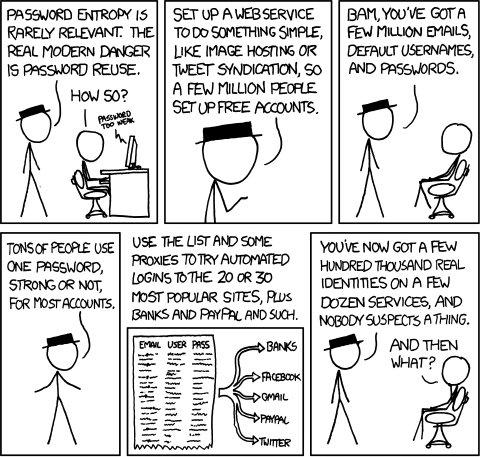
\includegraphics[height=0.8\textheight]{images/password_reuse_top.png}\\
  \end{center}
  \tiny Bildquelle: Ausschnitt aus \href{http://xkcd.com/792/}{xkcd: Password Reuse / CC BY-NC 2.5}
\end{frame}

\begin{frame}{Sichere Passwörter}
  \begin{block}{Anforderungen}
  \begin{itemize}
    \item Klein- und Großbuchstaben, Zahlen,\\ begrenzt: Sonderzeichen
    \item Wichtiger: Lang genug!
  \end{itemize}
  \end{block}
  \begin{block}{Merkbarkeit}
  \begin{itemize}
    \item Geschichte dazu ausdenken
    \item Melodie und Rhythmus rein bringen
    \begin{itemize}
      \item Gehirn kann sich Melodien besonders leicht merken
      \item Ermöglicht schnelles Eintippen
      \begin{itemize}
        \item Längere Passwörter sind weniger nervig
        \item Passwort mitlesen ist schwieriger
      \end{itemize}
    \end{itemize}
  \end{itemize}
  \end{block}
\end{frame}

\begin{frame}{Passwort-Manager}
  \begin{itemize}
    \item Software zur Verwaltung von Passwörtern
    \item Kann automatisch komplexe Passwörter erzeugen
    \item Datenbank wird mit Master-Passwort verschlüsselt
    \begin{itemize}
      \item Anzahl der zu merkenden Passwörter geringer
    \end{itemize}
    \item Beispiele
    \begin{itemize}
      \item KeePassX (Open Source)
      \item KeePass (Open Source)\\
        \textbf{Achtung:} Unsichere Update-Prüfung vor Version 2.34
    \end{itemize}
  \end{itemize}
  \begin{itemize}
    \item \emph{Wichtige Passwörter trotzdem merken\\oder an einem sicheren Ort aufbewahren!}
  \end{itemize}
\end{frame}

\endinput
